\subsection{Sekvensdiagrammer der anvendes i applikationsmodel for PSoC 5}
\begin{figure}[H]
	\caption{Sekvensdiagram for funktionen findEdge}
	\label{SD:PSoC:findEdge}
	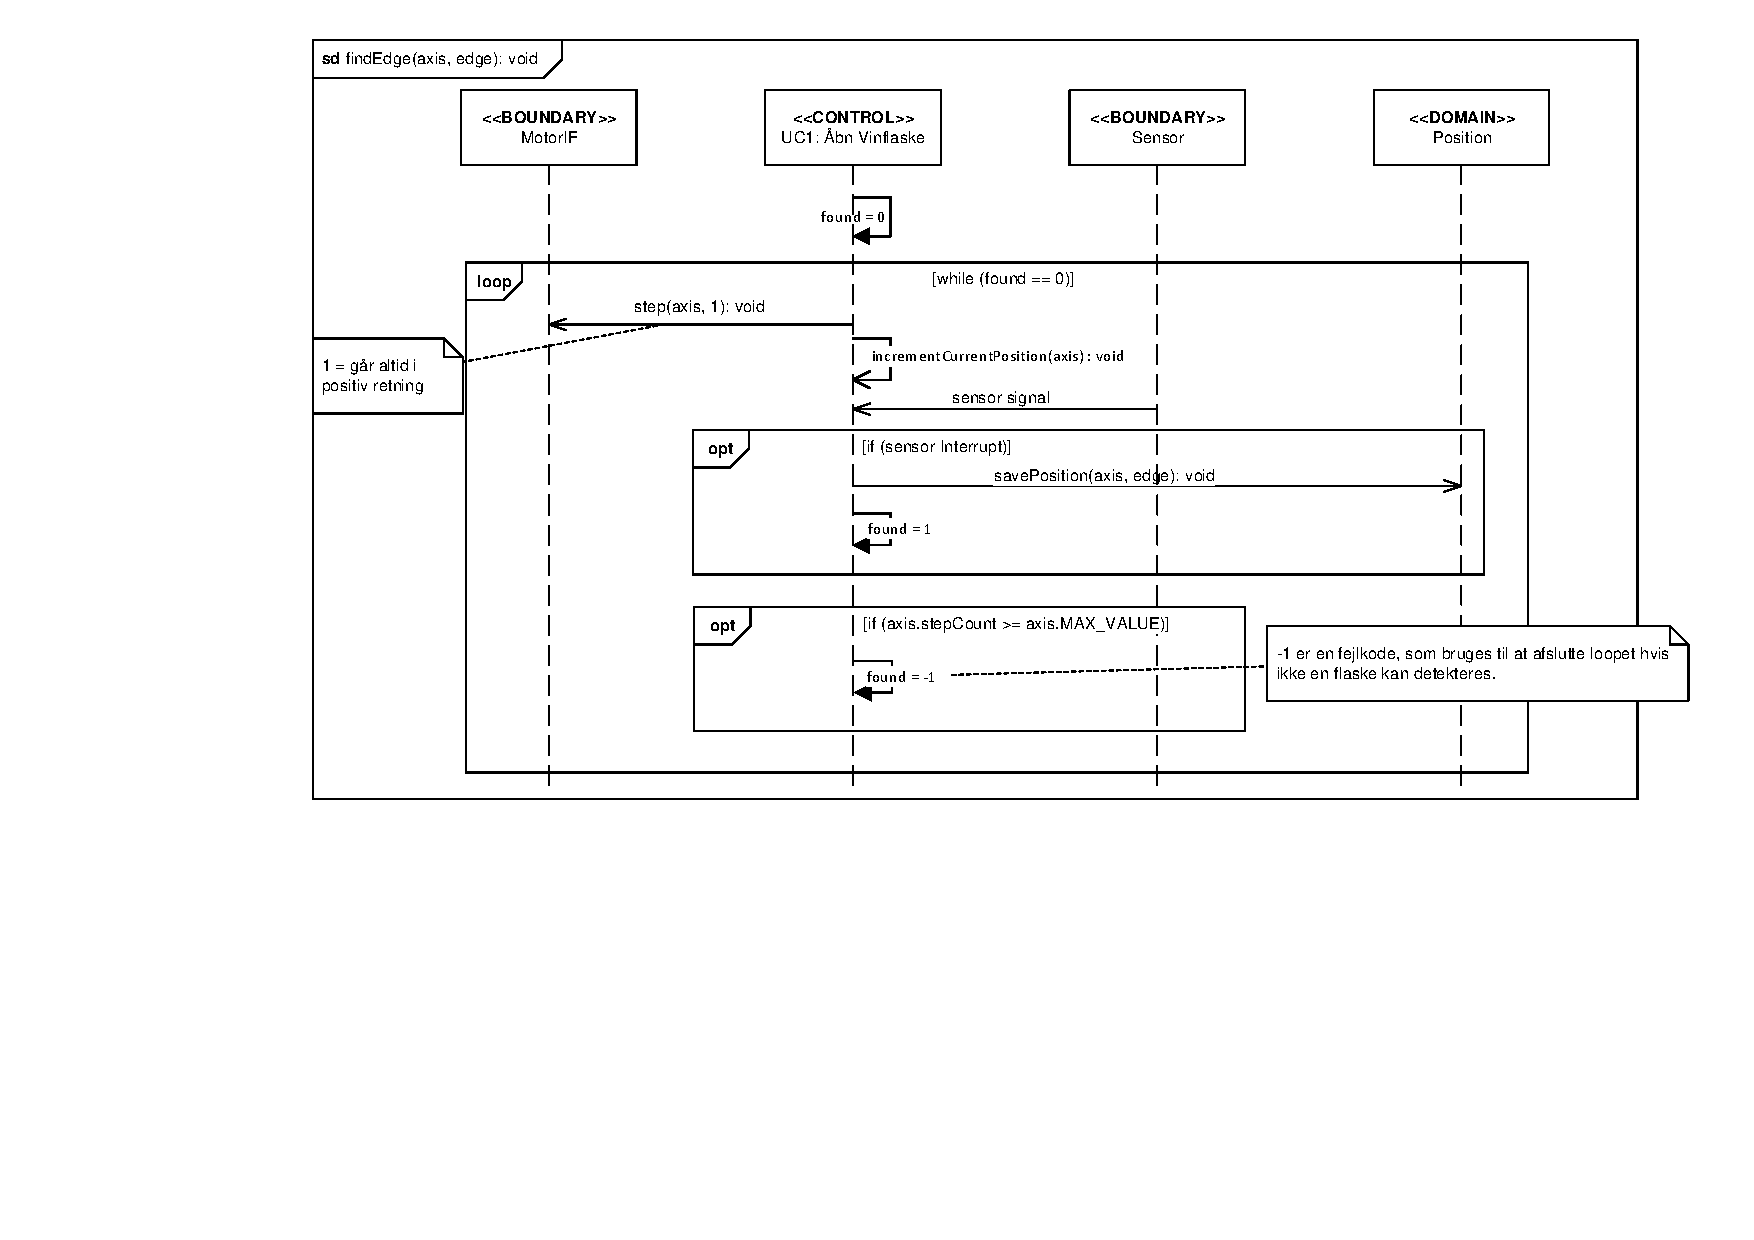
\includegraphics[scale=0.5,trim=100 0 0 0]{findEdge}
\end{figure}

\begin{figure}[H]
	\caption{Sekvensdiagram for funktionen opening process}
	\label{SD:PSoC:openingprocess}
	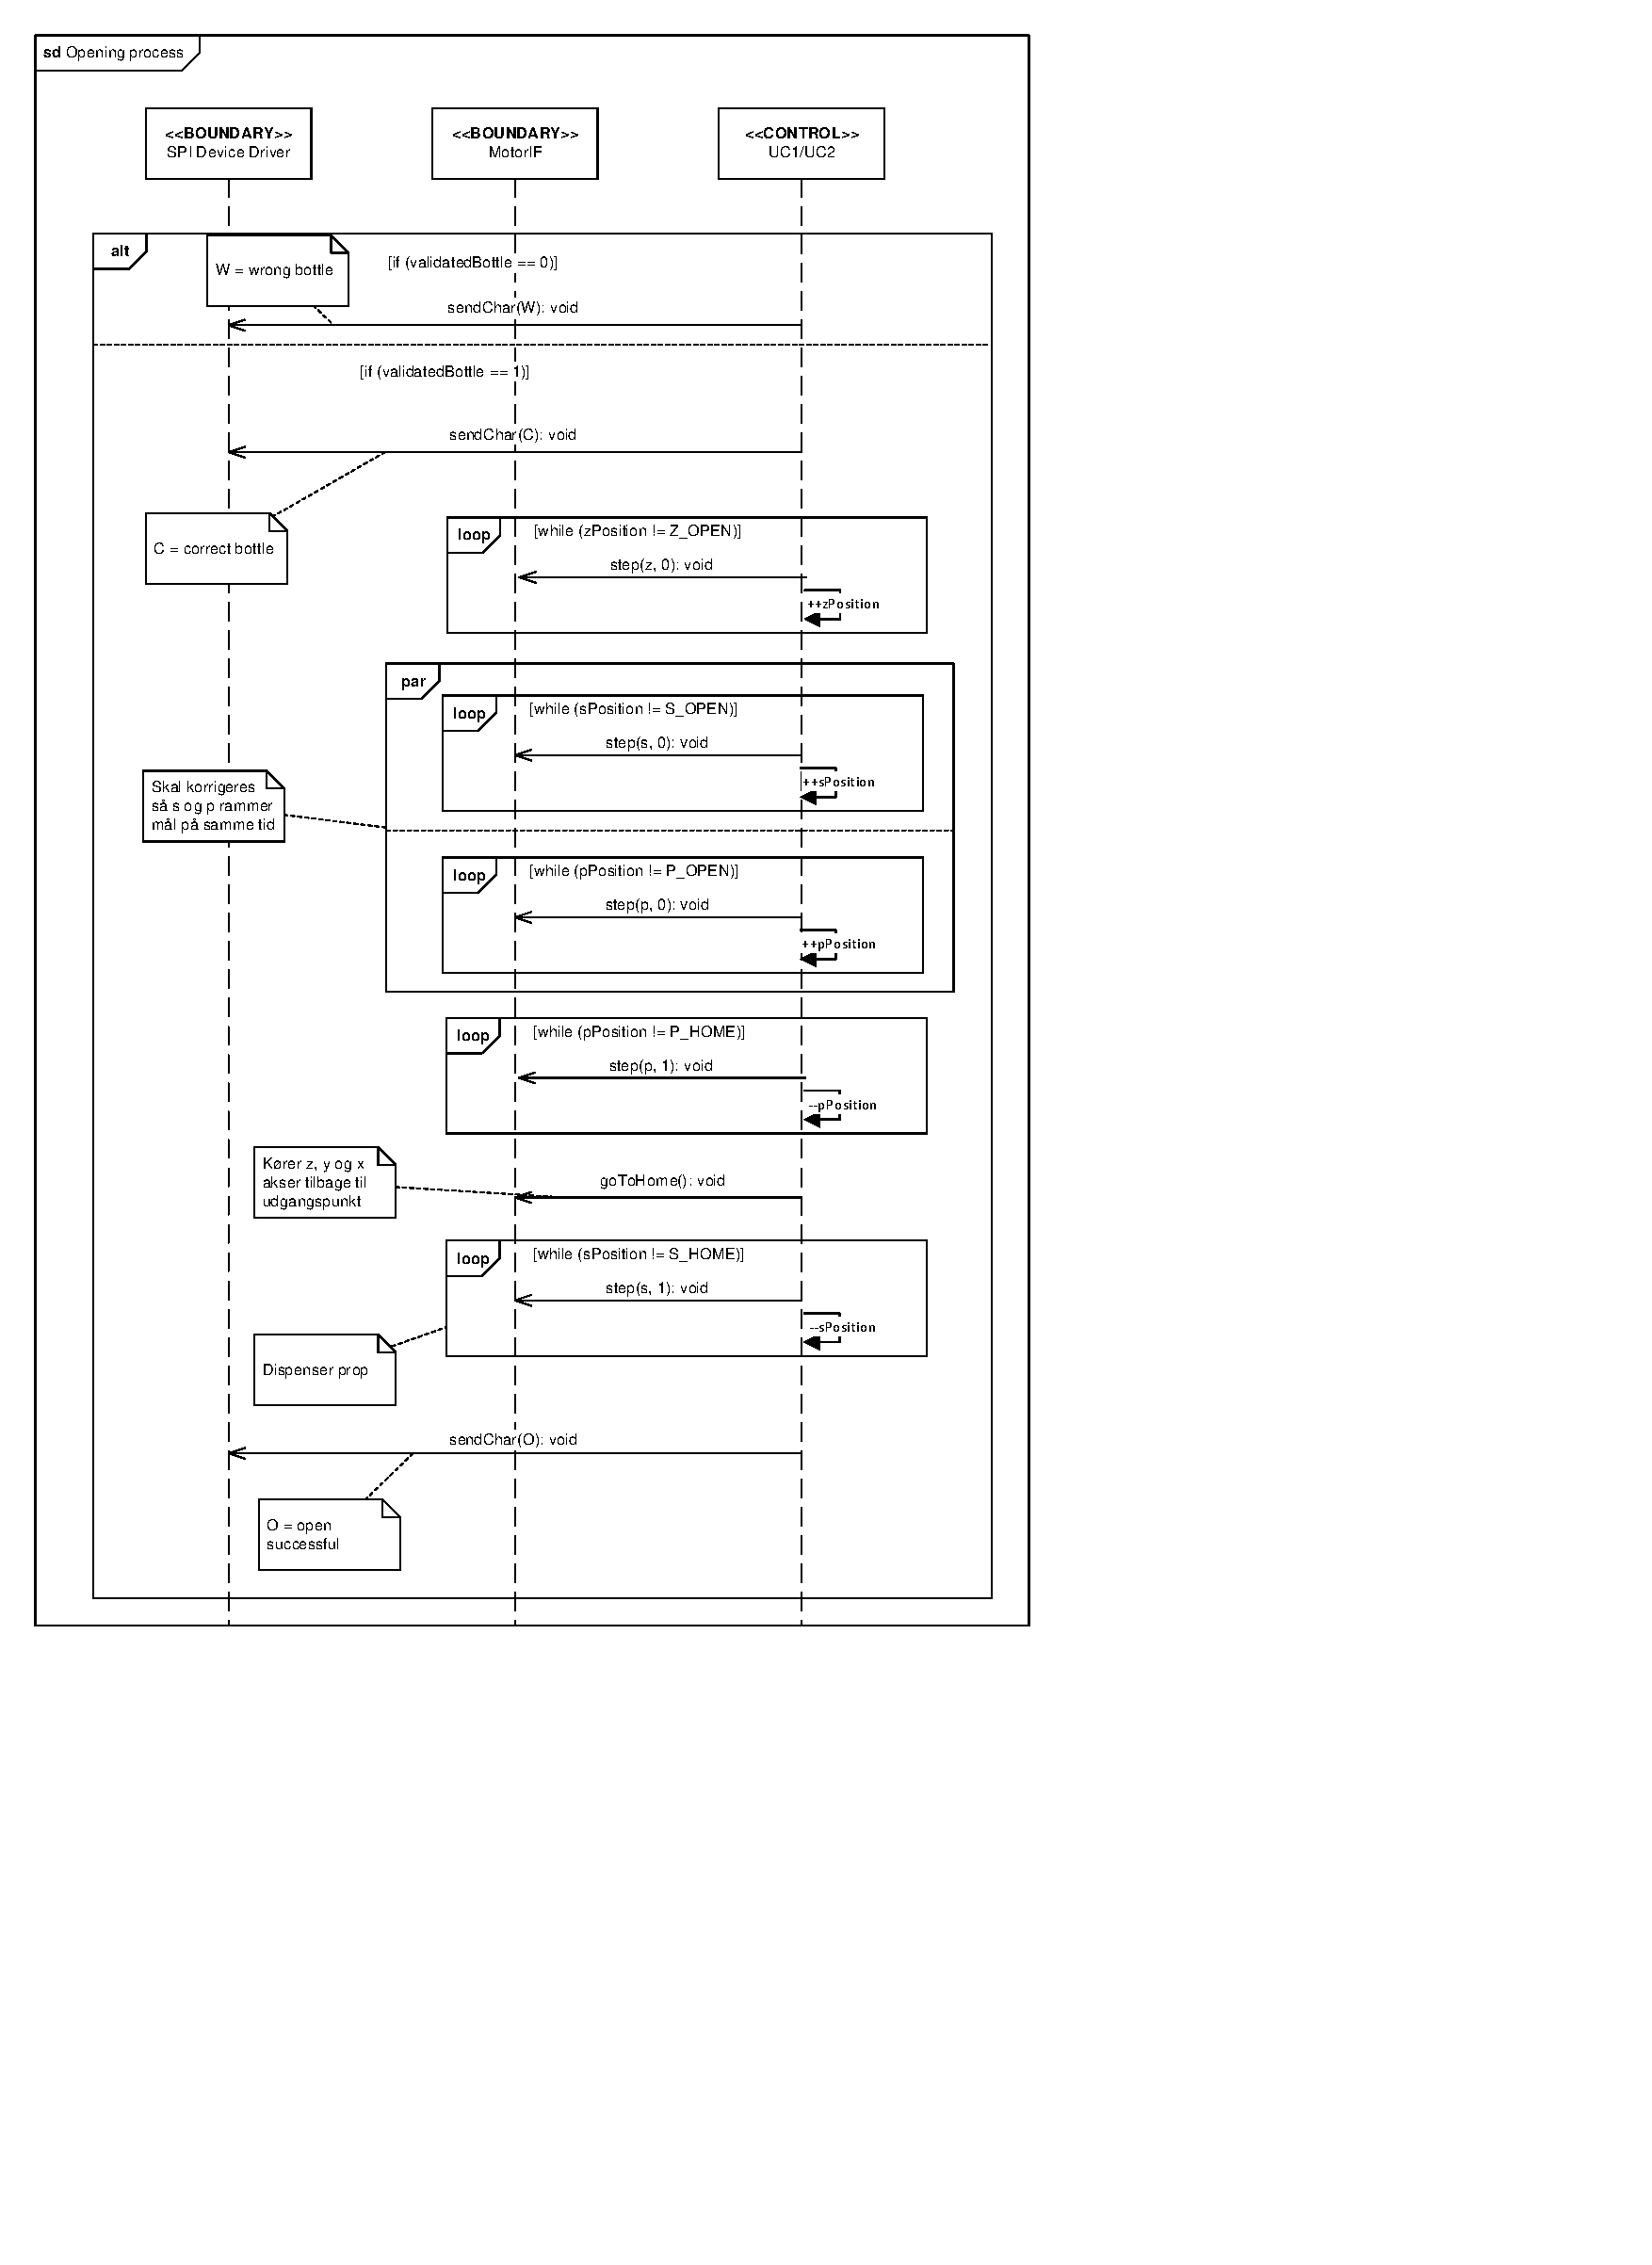
\includegraphics[scale=0.7,trim=0 0 0 0, clip]{Opening_process}
\end{figure}

%\begin{figure}[H]
%	\caption{Sekvensdiagram for funktionen Scan y-aksen}
%	\label{SD:PSoC:ScanY}
%	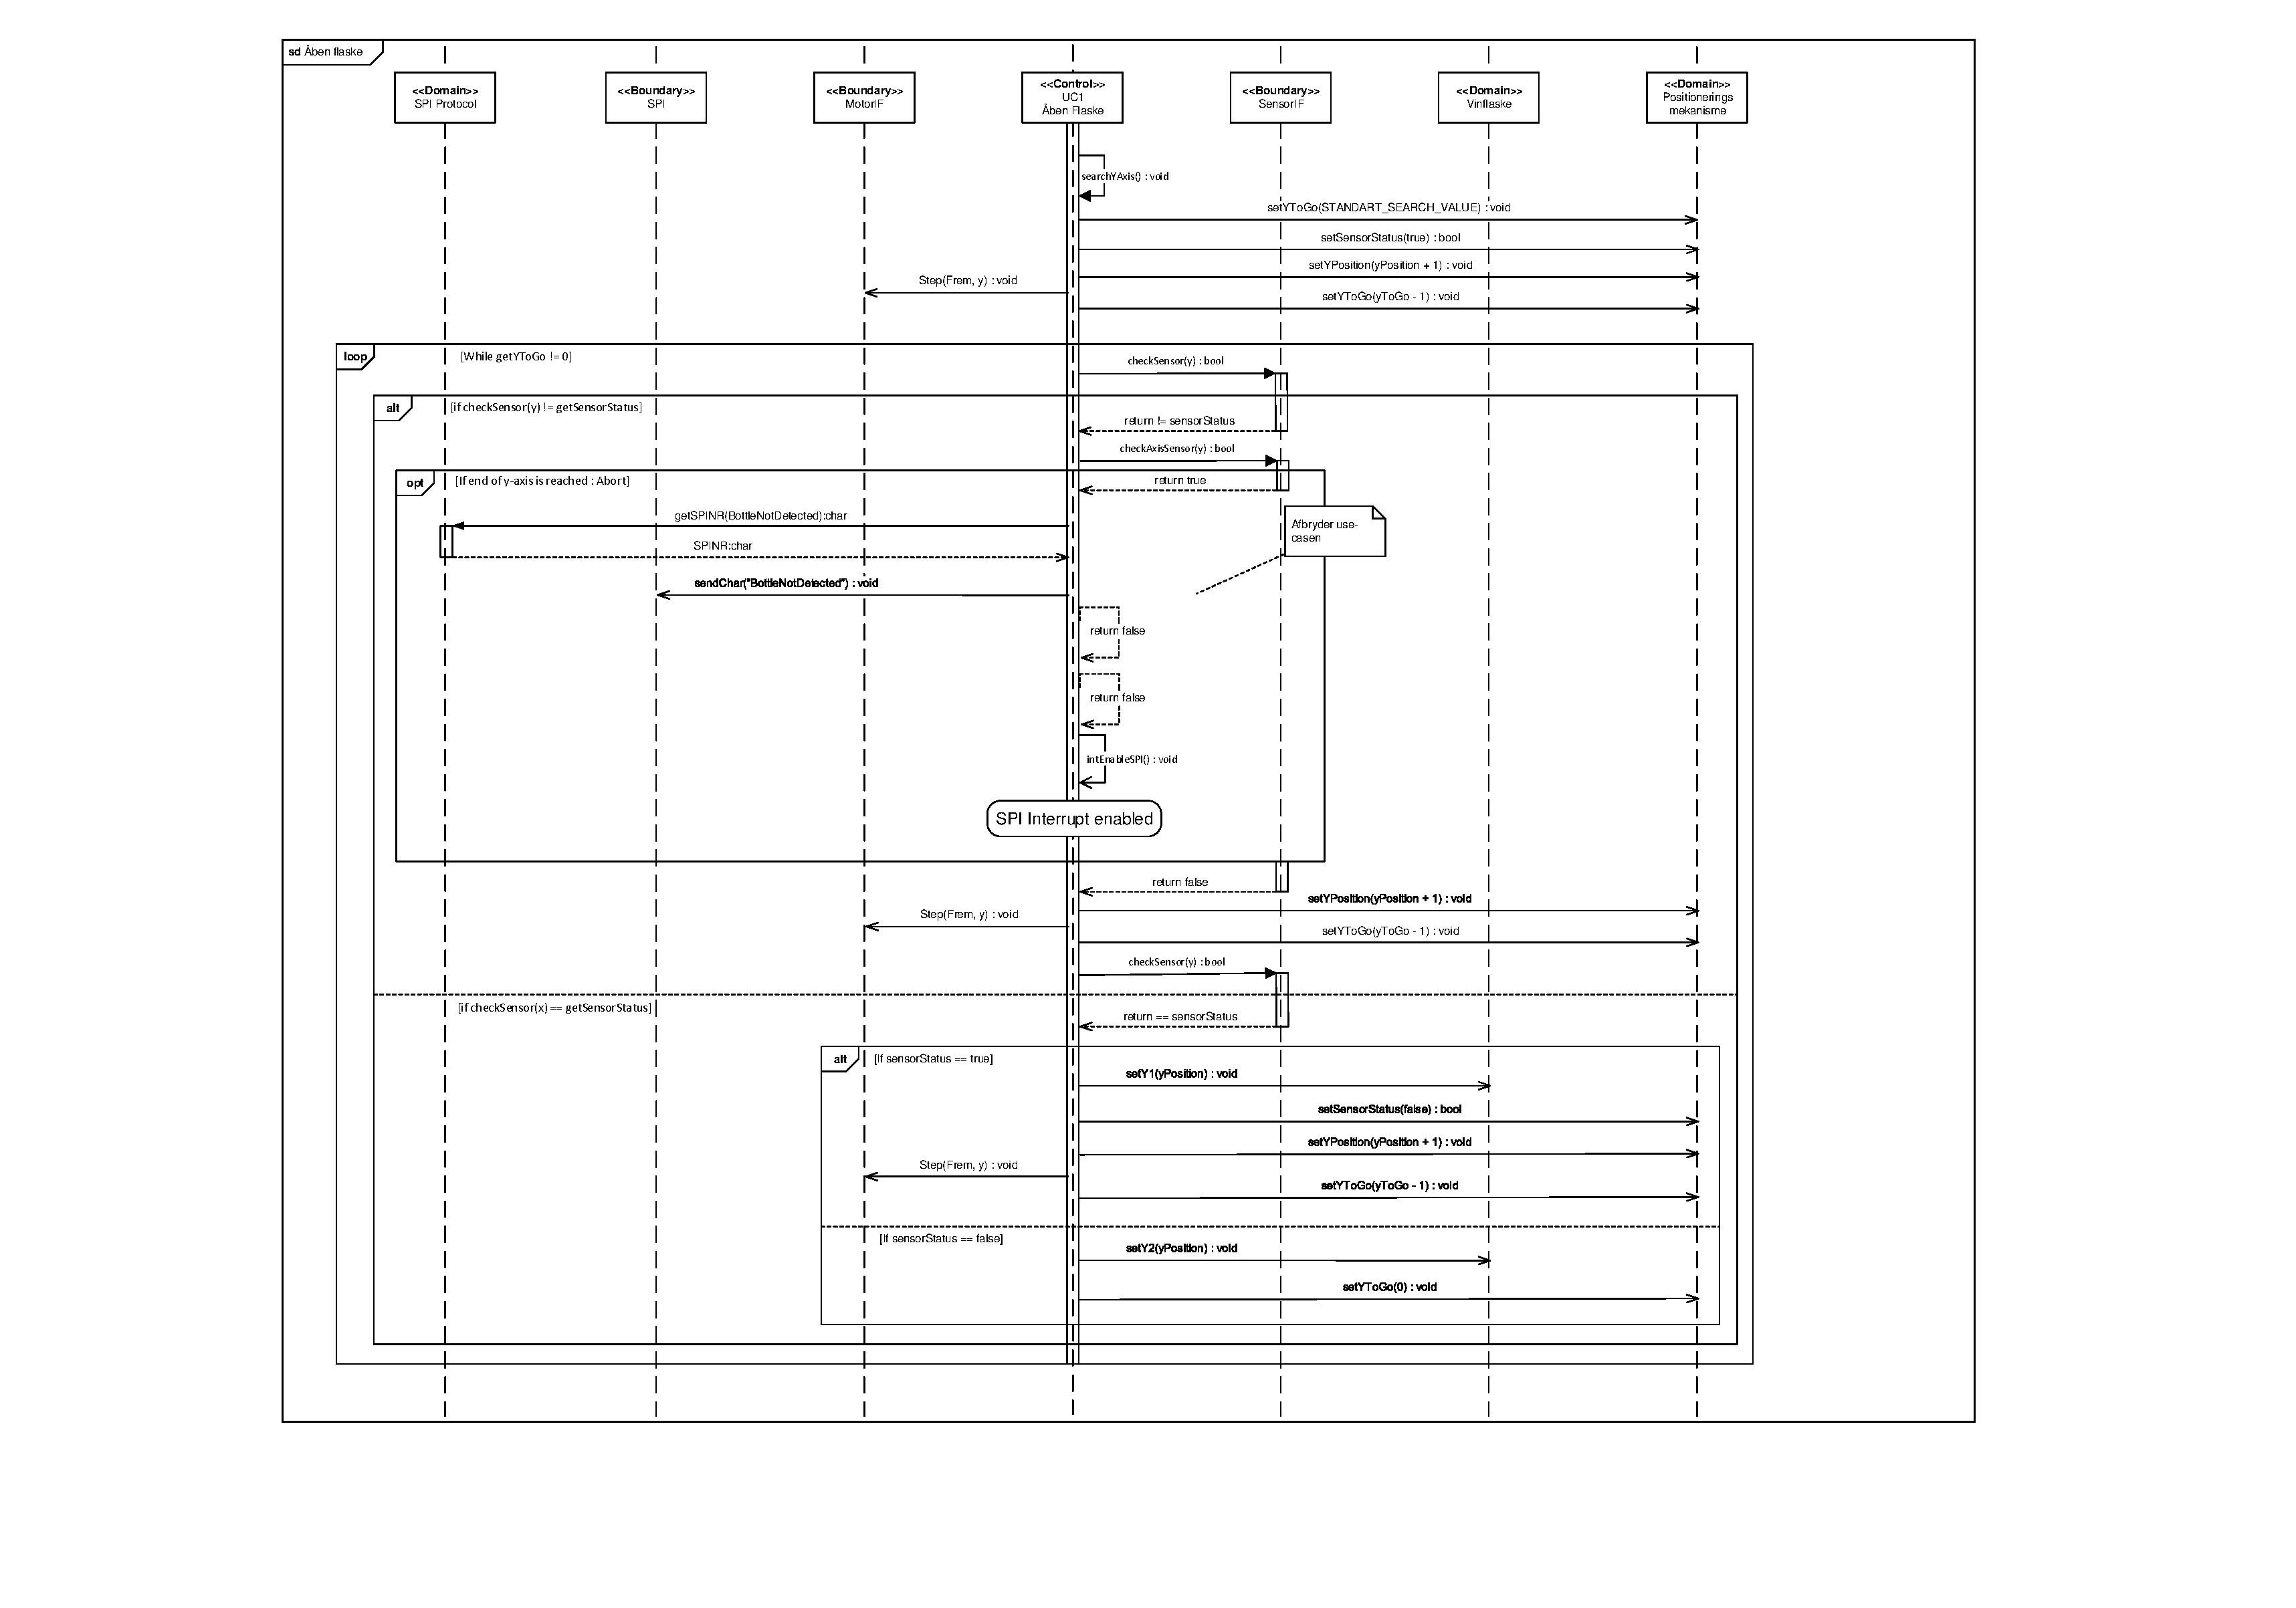
\includegraphics[scale=0.29,trim=200 100 0 0,clip]{APPSoC/SD-Scan-y-aksen}
%\end{figure}
%
%\begin{figure}[H]
%	\caption{Sekvensdiagram for funktionen Scan z-aksen}
%	\label{SD:PSoC:ScanZ}
%	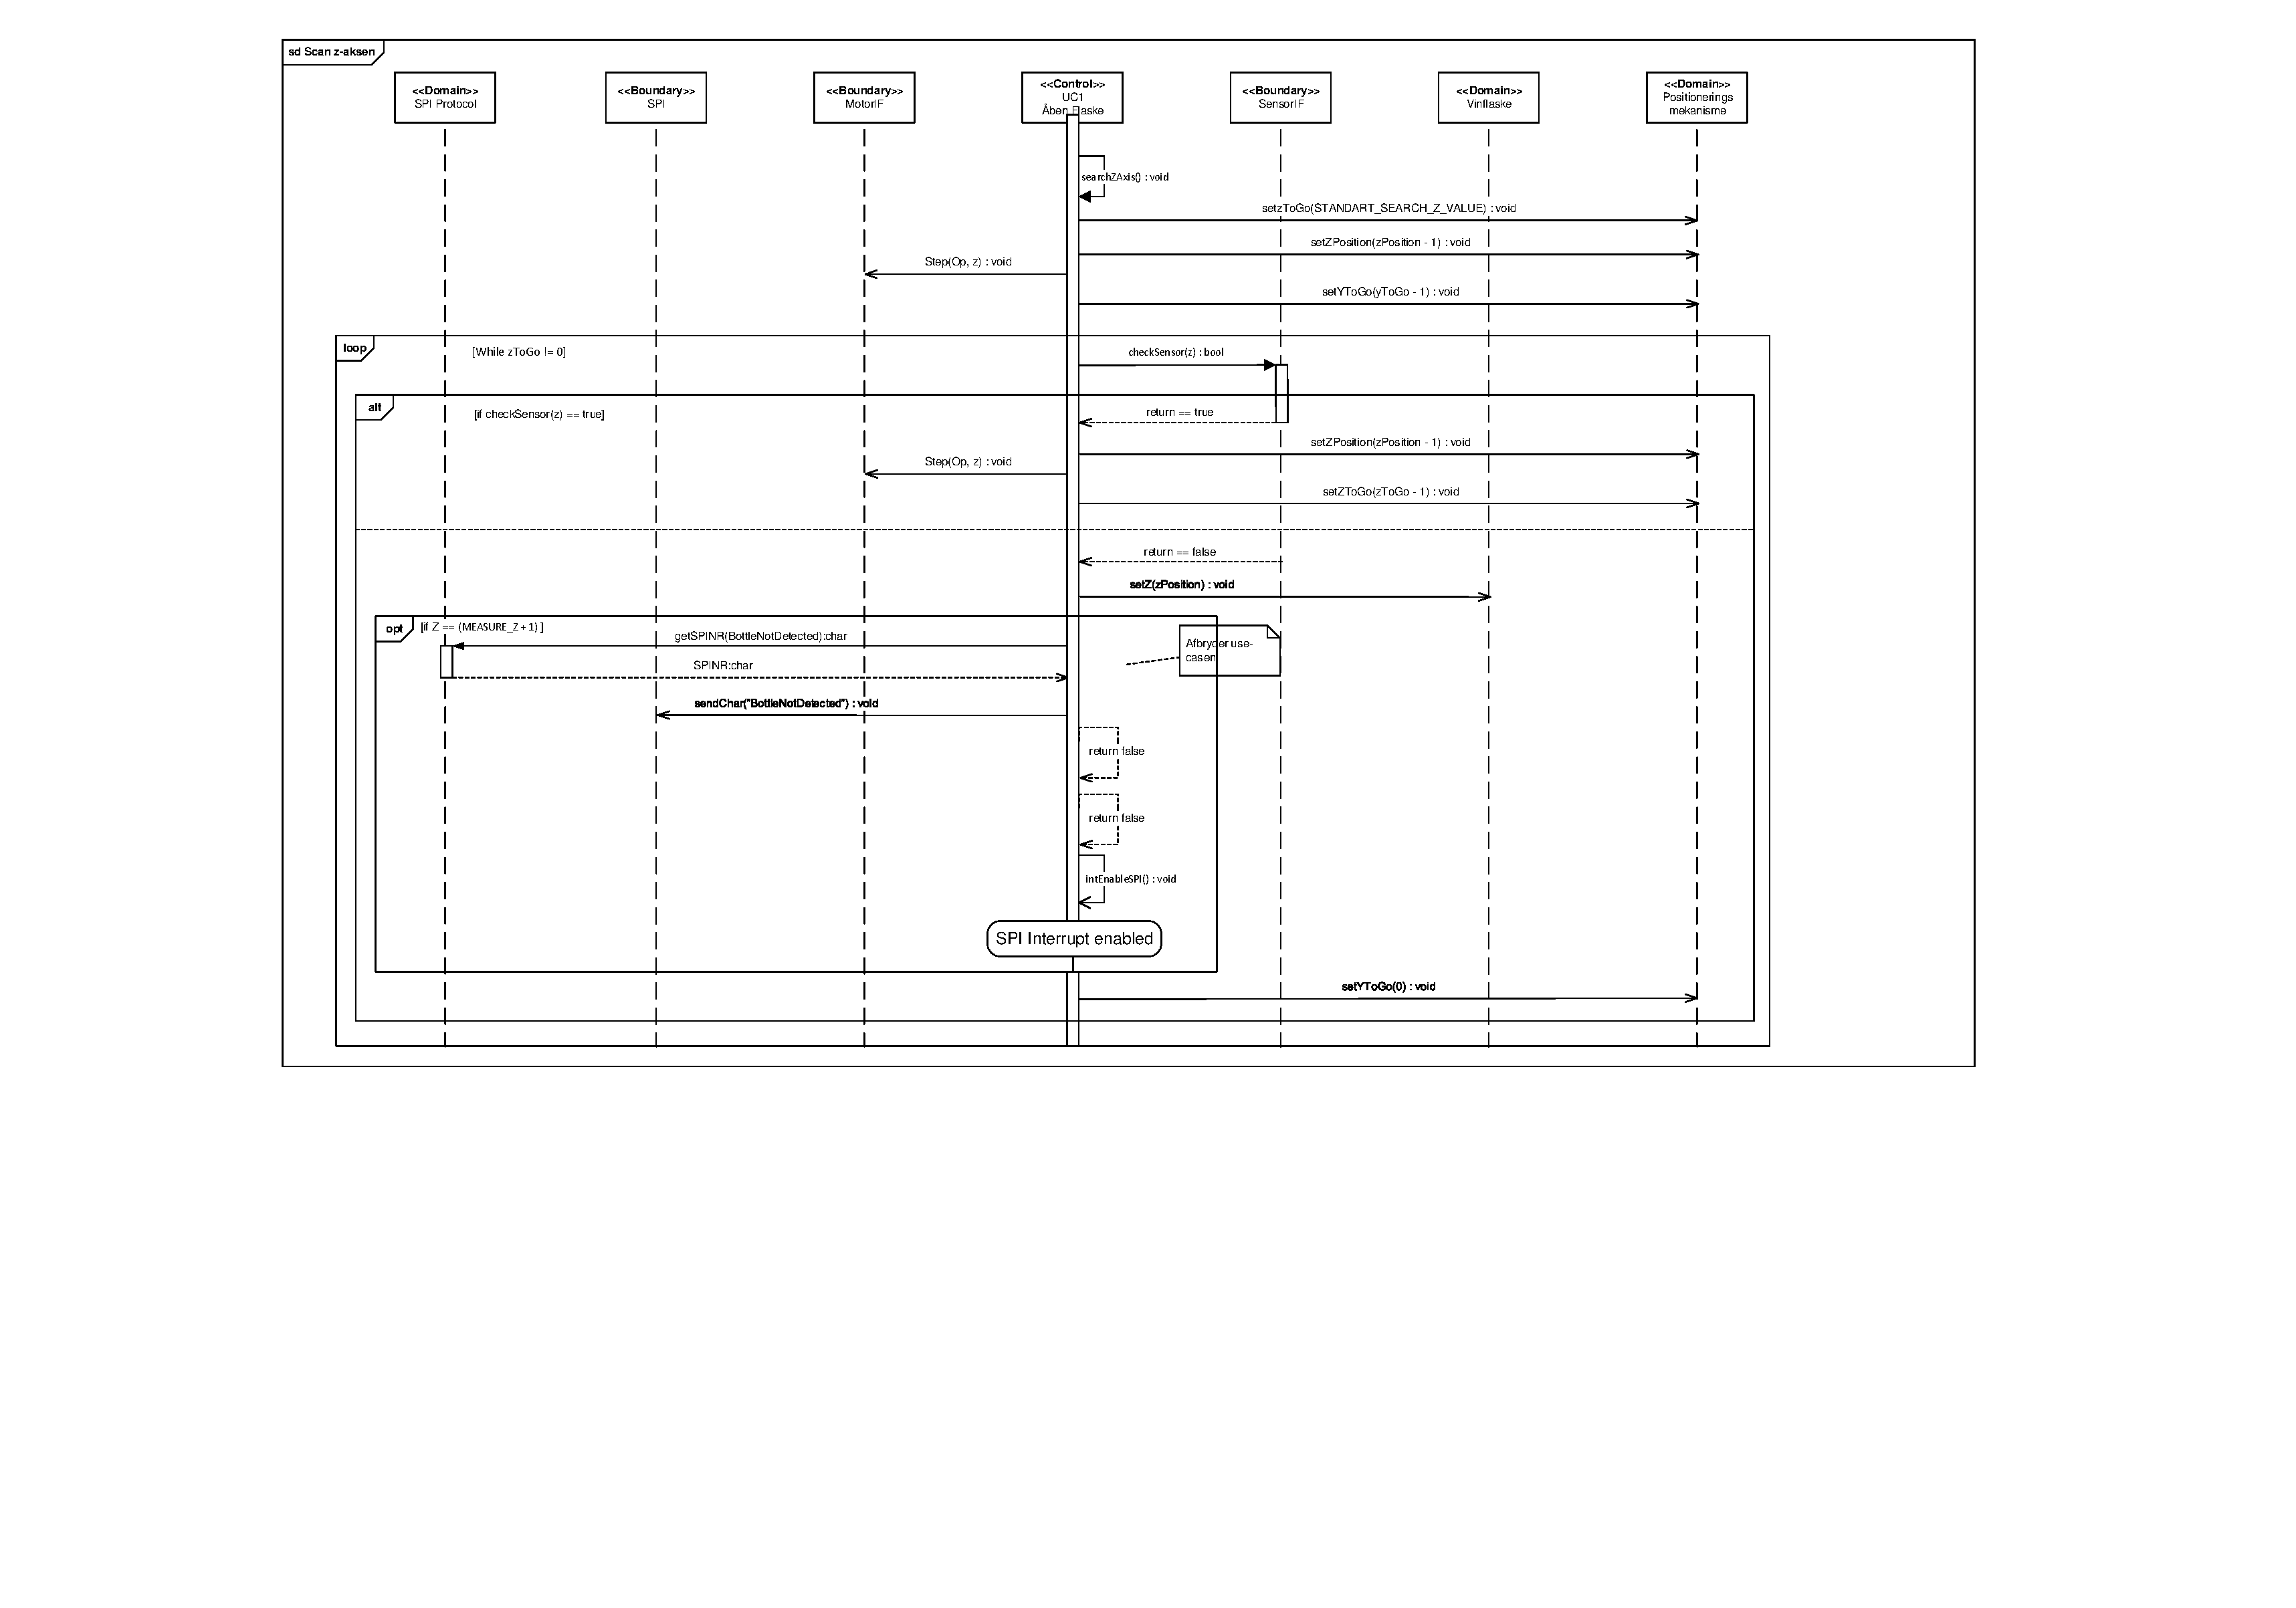
\includegraphics[scale=0.29,trim=200 100 0 0, clip]{APPSoC/SD-Scan-z-aksen}
%\end{figure}